\scanpage{37}
\[
H^1\bigl(X,\underbrace{\underline{\operatorname{Ext}}^1(f^*(B),G_{mX})}\bigr)
\]
\margin{\unsure{.\ '}}
\diagram{\begin{tikzcd}[ampersand replacement=\&, column sep=large,row sep=large]
\operatorname{Ext}_X(\overbrace{f^*(B)}^{A},G_{mX})\simeq\operatorname{Ext}_S(B,f_!(G_{mX}))\\
H^p(X,\underline{\operatorname{Ext}}^q_X(A,G_{mX})) \arrow[u,Rightarrow]
\end{tikzcd}}

\figure{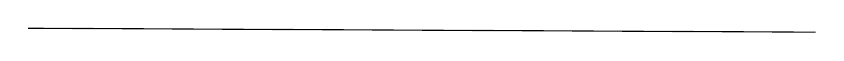
\begin{tikzpicture}\draw (0,.05)--(10,0);\end{tikzpicture}}

Suite exacte de Cohomologie. Critère de \unsure{surjectivité};

\unsure{Fibré universel}

Dualité de Cartier [voir \unsure{Pic.}\ldots]

Th. \unsure{projectivité} des V.A. (Th. de rigidité)

Propriétés \unsure{finicielles|fonctorielles} des groupes \ldots

Propriétés différentielles des \unsure{gpes} et fibrés

En particulier : \uuline{fibrés linéaires}, symplectiques, orthogonaux etc \ldots

\figure{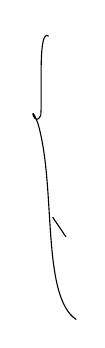
\begin{tikzpicture}\draw (0,3.6) .. controls (-.14,3.7) and (-.08,2.9) .. (-.1,2.6) .. controls (-.18,2.4) and (-.26,2.8) .. (-.14,2.5) .. controls (.1,1.7) and (-.1,.3) .. (.35,0);\draw (.05,1.3)--(.22,1.05);\end{tikzpicture}}

\unsure{Leur dualité} \unsure{pour} les \unsure{représentations lin. de groupes} ??

\figure{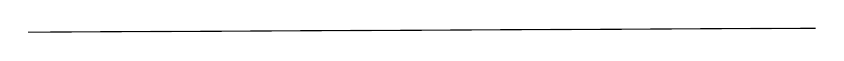
\begin{tikzpicture}\draw (0,0)--(10,.05);\end{tikzpicture}}
\[
\deleted{\underline{\operatorname{Hom}}(G_a,G_m)}
\]
\[
\mathbb Z.\quad\unsure{\vdash|\mapsto}\quad\mathbb Z
\]
\margin{36}
